%! Author = aybehrouz
%! Date = 2/28/21

% Preamble
\documentclass[11pt, A4]{report}

% Packages
%\usepackage{amsmath}
\usepackage{graphicx}
\graphicspath{ {../img/} }
\usepackage{hyperref}
\usepackage{amsfonts}
\usepackage[ruled,boxed]{algorithm2e}
\usepackage{algpseudocode}
\usepackage{listings}
\usepackage{amssymb}
\lstset{
%  basicstyle=\ttfamily,
    mathescape
}
%\binoppenalty=99999
%\relpenalty=99999

\title{The Argennon Virtual Machine}
\author{aybehrouz}
\date{January 2021}

% Document
\begin{document}
    \maketitle


    \chapter{Specification}\label{ch:specification}


    \section{Introduction}\label{sec:introduction}

    The Argennon Virtual Machine (AVM) is an abstract computing machine for executing Argennon's smart contracts. It
    is designed in a way that it could be efficiently implemented in either hardware or software.


    \section{The Structure of the Argennon Virtual Machine}\label{sec:the-structure-of-the-algorand-virtual-machine}

    ...

    \subsection{Data Types}\label{subsec:data-types}

    The Argennon Virtual Machine expects that all type checking is done prior to run time, typically by a compiler,
    and does not have to be done by the Argennon Virtual Machine itself.

    The instruction set of the Argennon Virtual Machine distinguishes its operand types using instructions intended to
    operate on values of specific types. For instance, \texttt{iadd} assumes that its operands are two 64-bit integers.

    \subsection{The \texttt{PC} Register}\label{subsec:the-pc-register}

    ...

    \subsection{Call Stack}\label{subsec:call-stack}

    A call stack contains the information that is needed for restoring the state of the invoker of a method.

    \subsection{Memory Unit}\label{subsec:memory-unit}

    The Argennon Virtual Machine has a byte addressable memory which is divided into separate segments. Every segment
    belongs to a smart contract that has a unique \texttt{applicationID}. The AVM always has a single working memory
    segment and memory locations outside its current working segment can not be accessed. The only instructions which
    can change the current working segment are \texttt{invoke\_external}, \texttt{athrow} and return instructions.

    Every smart contract has its own memory segment. Hence, there is no way for a smart contract to access another
    smart contract's memory. Interaction between smart contracts is done using \texttt{invoke\_external} instruction,
    and a smart contract can invoke methods of another smart contract by this instruction.

    A memory segment consists of five data areas:
    \begin{itemize}
        \item Code Area
        \item Constant Area
        \item Local Frame
        \item Operand Stack
        \item Heap
    \end{itemize}
    All data areas except operand stack, have their own address space which starts from 0. Operand stack is a
    last-in-first-out (LIFO) stack and is not addressable. Every memory access instruction operates on its specific
    data areas.

    \subsubsection{Code Area}

    The code area of a segment contains the byte-code of the smart contract which owns that segment. The AVM has no
    instructions for manipulating the code area. \textbf{Installing, removing and updating smart contracts need to
    be done externally.}

    \subsubsection{Constant Area}

    The constant area of a segment contains several kinds of constants, ranging from user defined constants to method
    address tables. A method address table stores method locations in the code area and their access type. The access
    type of a method can be either \texttt{public} or \texttt{private}. The AVM has no instructions for modifying the
    constant area.

    \emph{Only public methods can be invoked by \texttt{invoke\_external} instruction.}

    \subsubsection{Local Frame}

    A local frame is used to store methods parameters and local variables. A new frame is created each time a method
    is invoked, and it is destroyed when its method invocation completes, whether the completion is normal or abrupt.

    \subsubsection{Operand Stack}

    Every time a local frame is created, a corresponding empty last-in-first-out (LIFO) stack is created too. AVM
    instructions take operands from the operand stack, operate on them, and push the result back onto the operand
    stack. An operand stack is destroyed when its owner method completes, whether that completion is normal or abrupt.

    \subsubsection{Heap}

    The heap of a segment is a persistent memory area which is divided into pages. Memory locations inside every page
    have a separate address space that starts from 0, and each page can be referenced by an index that starts from 0. In
    other words, the address of every memory location inside a heap is a pair of indices: \texttt{(pageIndex, offset)}.
    Different pages of a heap do not need to be equally sized.

    \emph{The reason behind this paged design is that the heap is usually persisted using a block device. A heap with
    a paged structure could expose the underlying block based nature of the persistence layer to the application
    layer. In this way, the compiler or the programmer could better optimize the code for the persistence layer.}


    \section{Instruction Set Summary}\label{sec:instruction-set-summary}

    An Argennon Virtual Machine instruction consists of a \textbf{one-byte} opcode specifying the operation to be
    performed, followed by zero or more operands supplying arguments or data that are used by the operation.
    \textbf{The number and size of the operands are determined solely by the opcode.}

    \subsection{Method Invocation}\label{subsec:method-invocation}

    The Argennon Virtual Machine has three types of method invocation:
    \begin{itemize}
        \item \texttt{invoke\_internal} invokes a method from the current running smart contract.
        \item \texttt{invoke\_external} invokes a \texttt{public} method from another smart contract. It will change
        the current memory segment to the segment of the invoked smart contract.
        \item \texttt{invoke\_native} invokes a method that is not hosted by the Argennon virtual machine. By this
        instruction, high performance native methods of the hosting machine could become available to AVM smart
        contracts.
    \end{itemize}

    \emph{In the future, we may need to add special instructions for invoking interface and virtual methods...}

    Each time a method is invoked a new local frame and operand stack is created. The Argennon Virtual Machine uses
    local frames to pass parameters on method invocation. On method invocation, any parameters are passed in
    consecutive local variables stored in the method's local frame starting from local variable 0. The invoker of a
    method writes the parameters in the local frame of the invoked method using \texttt{arg} instructions.

    \subsubsection{Exceptions}

    An exception is thrown programmatically using the \texttt{athrow} instruction. Exceptions can also be thrown by
    various Argennon Virtual Machine instructions if they detect an abnormal condition. Some exceptions are not
    catchable and will always abort the execution of the smart contract.

    \subsubsection{Method Invocation Completion}

    A method invocation completes normally if that invocation does not cause an exception to be thrown, either
    directly from the AVM or as a result of executing an explicit throw statement. If the invocation of the current
    method completes normally, then a value may be returned to the invoking method. This occurs when the invoked
    method executes one of the return instructions, the choice of which must be appropriate for the type of the value
    being returned (if any). Execution then continues normally in the invoking method's local frame with the returned
    value (if any) pushed onto the operand stack.

    A method invocation completes abruptly if an exceptions is thrown and is not caught by the current method. A
    method invocation that completes abruptly never returns a value to its invoker.

    When a method completes, whether normally or abruptly, the call stack is used to restore the state of the invoker,
    including its local frame and operand stack, with the \texttt{PC} register appropriately restored and incremented
    to skip past the method invocation instruction. If the invoker was another smart contract, i.e.\ the invocation
    was made by an \texttt{invoke\_external} instruction, the current memory segment will be changed to the invoker's
    segment.

    A thrown exception causes methods in the call stack to complete \textbf{abruptly} one by one, as long as the
    \texttt{PC} register is not pointing to a \texttt{catch} instruction. The \texttt{catch} instruction acts like a
    branch instruction that branches only if an exception is caught. \textbf{When an external method invocation
    completes abruptly, before changing the current segment, all changes made to the heap area by that method
    call, including changes made to other segments, will be rolled back.} So, when a method call completes abruptly,
    that method call essentially has no effect on the AVM state.

    \emph{By using the \texttt{athrow} instruction properly, a programmer can make any method act like an atomic
    operation.}

    \subsection{Authorizing Operations}\label{subsec:authorizing-operations}

    In blockchain applications, we usually need to authorize certain operations. For example, for sending an asset
    from a user to another user, first we need to make sure that the sender has authorized this operation. The
    Argennon virtual machine has no built in mechanism for authorizing operations, but it provides a rich set of
    cryptographic instructions for validating signatures and cryptographic entities. By using these instructions and
    passing signatures as parameters to methods, a programmer can implement the required logic for authorizing any
    operation.

    \emph{The Argennon virtual machine has no instructions for issuing cryptographic signatures.}

    In addition to signatures, a method can verify its invoker by using \texttt{get\_parent} instruction. This
    instruction gets the \texttt{applicationID} of the smart contract that is one level deeper than the current
    smart contract in the call stack. In other words, it returns the \texttt{applicationID} of the smart contract that
    has invoked the current smart contract. (if any)

    \subsection{Heap Allocation Instructions}\label{subsec:heap-allocation-instructions}

    ...


    \section{The AVM Standard Library}\label{sec:the-avm-standard-library}

    ...


    \chapter{Implementation}\label{ch:implementation}


    \section{Persistence}\label{sec:persistence}

    For implementing the persistence layer of the AVM, we assume that we have access to an updatable zero-knowledge
    elementary database (ZK-EDB) with the following properties:

    \begin{itemize}
        \item The ZK-EDB contains a mapping from a set of keys to a set of values.
        \item Every state of the database has a commitment \(C\).
        \item The ZK-EDB has a method \((D, p) = get(x)\), where \(x\) is a key and \(D\) is the associated data
        with \(x\), and \(p\) is a proof.
        \item A user can use \(C\) and \(p\) to verify that \(D\) is really associated with \(x\), and \(D\) is not
        altered. Consequently, a user who can obtain \(C\) from a trusted source does not need to trust the ZK-EDB.
        \item Having \(p\) and \(C\) a user can compute the commitment \(C'\) for the database in which \(D'\) is
        associated with \(x\) instead of \(D\).
    \end{itemize}

    We use a ZK-EDB for storing the AVM heap. We include the commitment of the current state of this DB in every
    block of the Argennon blockchain, so ZK-EDB servers need not be trusted servers.

    Every page of AVM heap will be stored with a key of the form: \texttt{applicationID|pageIndex} (the \texttt{|}
    operator concatenates two numbers). Nodes do not keep a full copy of the AVM heap and for validating block
    certificates or emulating the AVM ( i.e.~validating transactions) they need to connect to a ZK-EDB and retrieve
    the required pages of AVM heap. For better performance, nodes keep a cache of heap pages to
    reduce the amount of ZK-EDB access.

    We also use a ZK-EDB for storing the code area of each segment, and we include the commitment of this DB in every
    block. Every code area will be divided into blocks and every block will be stored in the DB with
    \texttt{applicationID|blockID} as its key. Like heap pages, nodes keep a cache of code area blocks.

    \emph{Unlike heap pages, the AVM is not aware of different blocks of code area.}


    \section{Transactions}\label{sec:transactions}

    Argennon has four types of transaction:

    \begin{itemize}
        \item \texttt{avmCall} essentially is an \texttt{invoke\_external} instruction that invokes a method from an
        AVM smart contract. Users interact with AVM smart contracts using these transactions. Transferring all
        assets, including ARGs, is done by these transactions.
        \item \texttt{installApp} installs an AVM smart contract and determines the update policy of the smart
        contract: if the contract is updatable or not, which accounts can update or uninstall the contract, and so
        on.
        \item \texttt{unInstallApp} removes an AVM smart contract.
        \item \texttt{updateApp} updates an AVM smart contract.
    \end{itemize}

    All types of Argennon transactions contain an \texttt{invoke\_external} instruction which calls a special method
    from ARG smart contract that transfers the proposed fee of the transaction in ARGs from a sender account to the
    fee sink accounts.

    Every transaction is required to exactly specify what heap locations or code area addresses it will access. This
    enables validators to start retrieving the required memory blocks from available ZK-EDB servers as soon as they
    see a transaction, and they won't need to wait for receiving the new proposed block. A transaction that tries to
    access a memory location that is not included in its access lists, will be rejected. Users could use smart contract
    oracles to predict the list of memory blocks their transactions need. See Section~\ref{sec:smart-contract-oracle}
    for more details.


    \section{Blockchain}\label{sec:blockchain}

    Every block of the Argennon blockchain corresponds to a set of transactions. We store the commitment of this
    transaction set in every block, but we don't keep the set itself. To be able to detect replay attacks, we require
    every signature that a user creates to have a nonce. This nonce consists of the issuance round of the signature
    and a sequence number: \texttt{(issuance,\ sequence)}. When a user creates more than one signature in a round, he
    must sequence his signatures starting from 0 (i.e.~the sequence number restarts from 0 in every round). We define
    a maximum lifetime for signatures, so a signature is invalid if \texttt{currentRound - issuance \textgreater{}\
        maxLifeTime} or if a signature of the same user with a bigger or equal nonce is already used
    (i.e.~is recorded in the blockchain). A nonce is bigger than another nonce if it has an older issuance. If two
    nonces have an equal issuance, the nonce with the bigger sequence number will be considered bigger.

    To be able to detect invalid signatures, we keep the maximum nonce of used digital signatures per user. When the
    difference between \texttt{issuance} component of this nonce and the current round becomes bigger than the
    maximum allowed lifetime of a signature, this information can be safely deleted. \textbf{As a result, we will not
    have the problem of "un-removable empty accounts" like Ethereum.}

    The only information that Argennon nodes are required to store is \textbf{the most recent block} of the Argennon
    blockchain. Every block of the Argennon blockchain contains the following information:

    \begin{center}
        \begin{tabular}{||c||}
            \hline
            Block \\ [0.5ex]
            \hline\hline
            commitment to the ZK-EDB storing heap pages \\ [0.7ex]
            commitment to the ZK-EDB storing code areas \\ [0.7ex]
            commitment to the set of transactions       \\ [0.7ex]
            previous block hash                         \\ [0.7ex]
            random seed                                 \\ [0.7ex]
            \hline
        \end{tabular}
    \end{center}

    For confirming a new block, nodes that are not validators only need to verify the block certificate. For
    verifying a block certificate, a node needs to know the ARG balances of validators, but it doesn't need to
    emulate the AVM execution.

    On the other hand, nodes that are chosen to be validators, for validating a new block, need to emulate the
    execution of the Argennon virtual machine. To do so, first they retrieve all heap pages and code area blocks they
    need from available ZK-EDBs. Then, they emulate the execution of AVM instructions and validate all the
    transactions included in the new block. This will modify some pages of the AVM memory, so they update the ZK-EDB
    commitments based on the modified pages and verify the commitments included in the new block. Validators also
    calculate and verify the commitment to the new block's transaction set.

    \emph{Validators do not need to write the modified pages back to ZK-EDB servers. ZK-EDBs will receive the new
    block, and they will update their database by emulating the AVM execution.}


    \section{Incentive mechanism}\label{sec:incentive-mechanism}

    \subsection{Transaction Fee}\label{subsec:transaction-fee}

    Every transaction in the Argennon blockchain starts with an \texttt{invoke\_external} instruction which calls a
    special method from ARG smart contract. This method will transfer the proposed fee of the transaction in ARGs
    from a sender account to the fee sink accounts. Argennon has two fee sink accounts: \texttt{execFeeSink} collects
    execution fees and \texttt{dbFeeSink} collects fees for ZK-EDBs. The Protocol decides how to distribute the
    transaction fee between these two fee sink accounts.

    When a block is added to the blockchain, the proposer of that block will receive a share of the block fees.
    Consequently, a block proposer is always incentivized to include more transactions in his block. However, if he
    puts too many transactions in his block and the validation of the block becomes too difficult, some validators
    may not be able to validate all transactions on time. If a validator can not validate a block in the required
    time, he will consider the block invalid. So, when a proposed block contains too many transactions, the network
    may reach consensus on another block, and the proposer of that block will not receive any fees. As a result, a
    proposer is incentivized to use network transaction capacity optimally.

    On the other hand, we believe that the proposer does not have enough incentives for optimizing the storage size
    of the transaction set. Therefore, we require that \textbf{the size of the transaction set of every block in
    bytes be lower than a certain threshold.}

    Validators need to spend resources for validating transactions. When a validator starts the emulation of the AVM
    to validate a transaction, solely from the code he can't predict the time the execution will finish. This will
    give an adversary an opportunity to attack the network by broadcasting transactions that never ends. Since,
    validators can not finish the execution of these transactions, the network will not be able to charge the
    attacker any fees, and he would be able to waste validators resources for free.

    To mitigate this problem, we require that every transaction specify a cap for all the resources it needs. This
    will include memory, network and processor related resources. Also, the protocol defines an execution cost for
    every AVM instruction reflecting the amount of resources its emulation needs. This will define a standard way for
    measuring the execution cost of any \texttt{avmCall} transaction. Every \texttt{avmCall} transaction is required
    to specify a maximum execution cost. If during emulation it reaches this maximum cost, the transaction will be
    considered failed and the network can receive the proposed fee of that transaction.

    Every \texttt{avmCall} transaction is required to provide the following information as an upper bound for the
    resources it needs:

    \begin{itemize}
        \item Execution cost
        \item A list of heap/code-area locations for reading
        \item A list of heap locations for writing
        \item A list of heap pages it will deallocate
        \item Number and size of heap pages it will allocate
    \end{itemize}

    If a transaction tries to violate any of these predefined limitations, for example, if it tries to read a memory
    location that is not included in its reading list, it will be considered failed and the network can receive the
    proposed fee of that transaction.

    \emph{A transaction always pays all of its proposed fee, no matter how much of its predefined resources were not
    used in the final emulation.}

    \subsection{ZK-EDB Servers}\label{subsec:zk-edb-servers}

    The incentive mechanism for ZK-EDB servers should have the following properties:

    \begin{itemize}
        \item It incentivizes storing all memory blocks, whether a heap page or a code area block, and not only those
        which are used more frequently.
        \item It incentivizes ZK-EDB servers to actively provide the required memory blocks for validators.
        \item Making more accounts will not provide any advantages for a ZK-EDB server.
    \end{itemize}

    For our incentive mechanism, we require that every time a validator receives a memory block from a ZK-EDB, after
    validating the data, he give a receipt to the ZK-EDB. In this receipt the validator signs the following information:

    \begin{itemize}
        \item \texttt{ownerAddr}: the ARG address of the ZK-EDB\@.
        \item \texttt{receivedBlockID}: the ID of the received memory block.
        \item \texttt{round}: the current round number.
    \end{itemize}

    \emph{In a round, an honest validator never gives a receipt for an identical memory block to two different ZK-EDBs.}

    To incentivize ZK-EDB servers, a lottery will be held every round and a predefined amount of ARGs from
    \texttt{dbFeeSink} account will be distributed between winners as a prize. This prize will be divided equally
    between all \emph{winning tickets} of the lottery.

    \emph{One ZK-EDB server could own multiple winning tickets in a round.}

    To run this lottery, every round, based on the current block seed, a collection of \emph{valid} receipts will be
    selected randomly as the \emph{winning receipts} of the round. A receipt is \emph{valid} in the round \(r\) if:

    \begin{itemize}
        \item The signer was a validator in the round \(r - 1\) and voted for the agreed-upon block.
        \item The data block in the receipt was needed for validating the \textbf{previous} block.
        \item The receipt round number is \(r - 1\).
        \item The signer did not sign a receipt for the same data block for two different ZK-EDBs in the previous round.
    \end{itemize}
    For selecting the winning receipts we could use a random generator:
    \begin{verbatim}
IF random(seed|validatorPK|receivedBlockID) < winProbability THEN
    the receipt issued by validatorPK for receivedBlockID is a winner
    \end{verbatim}
    \begin{itemize}
        \item \texttt{random()} produces uniform random numbers between 0 and 1, using its input argument as a seed.
        \item \texttt{validatorPK} is the public key of the signer of the receipt.
        \item \texttt{receivedBlockID} is the ID of the memory block that the receipt was issued for.
        \item \texttt{winProbability} is the probability of winning in every round.
        \item \texttt{seed} is the current block seed.
        \item \texttt{|} is a concatenation operator.
    \end{itemize}

    \emph{The winners of the lottery were validators one round before the lottery round.}

    Also, based on the current block seed, a random memory block, whether a heap page or a code area block, is
    selected as the challenge of the round. A ZK-EDB that owns a winning receipt needs to broadcast a \emph{winning
    ticket} to claim his prize. The winning ticket consists of a winning receipt and a \emph{solution} to the round
    challenge. Solving a round challenge requires the content of the memory block which was selected as the round
    challenge. This will encourage ZK-EDBs to store all memory blocks.

    A possible choice for the challenge solution could be the cryptographic hash of the content of the challenge
    memory block combined with the ZK-EDB ARG address: \texttt{hash(challenge.content|ownerAddr)}

    The winning tickets of the lottery of the round \(r\) need to be included in the block of the round \(r\),
    otherwise they will be considered expired. Validation and prize distribution for the winning tickets of the round
    \(r\) will be done in the round \(r + 1\). This way, \textbf{the content of the challenge memory block could be
    kept secret during the lottery round.} Every winning ticket will get an equal share of the lottery prize.

    \subsection{Memory Allocation and De-allocation}\label{subsec:memory-allocation-and-de-allocation}

    Every \(k\) round the protocol chooses a price per byte for AVM memory. When a smart contract executes a heap
    allocation instruction, the protocol will automatically deduce the cost of the allocated memory from the ARG
    address of the smart contract.

    To determine the price of AVM memory, Every \(k\) round, the protocol calculates \texttt{dbFee} and
    \texttt{memTraffic} values. \texttt{dbFee} is the aggregate amount of collected database fees, and
    \texttt{memTraffic} is the total memory traffic of the system. For calculating the memory traffic of the system
    the protocol considers the total size of all the memory pages that were accessed for either reading or writing
    during a time period. These two values will be calculated for the last \(k\) rounds and the price per byte of
    AVM memory will be a linear function of \texttt{dbFee/memTraffic}

    When a smart contract executes a heap de-allocation instruction, the protocol will refund the cost of
    de-allocated memory to the smart contract. Here, the current price of AVM memory does not matter and the protocol
    calculates the refunded amount based on the average price the smart contract had paid for that allocated memory.
    This will prevent smart contracts from profit taking by trading memory with the protocol.


    \section{Concurrency}\label{sec:concurrency}

    \subsection{Memory Dependency Graph}\label{subsec:memory-dependency-graph}

    Every block of the Argennon blockchain contains a list of transactions. This list is an ordered list and the
    effect of its contained transactions must be applied to the AVM state sequentially as they appear in the ordered
    list. This ordering is solely chosen by the block proposer, and users should not have any assumption about
    the ordering of transactions in a block.

    The fact that block transactions constitute a sequential list, does not mean they can not be executed and applied
    to the AVM state concurrently. Many transactions are actually independent and the order of their execution does not
    matter. These transactions can be safely validated in parallel by validators.

    A transaction can change the AVM state by modifying either the code area or the AVM heap. In Argennon, all
    transactions declare the list of memory locations they want to read or write. This will enable us to determine the
    independent sets of transactions which can be executed in parallel. To do so, we define the \emph{memory dependency
    graph} \(G_d\) as follows:

    \begin{itemize}
        \item \(G_d\) is an undirected graph.
        \item Every vertex in \(G_d\) corresponds to a transaction and vice versa.
        \item Vertices \(u\) and \(v\) are adjacent in \(G_d\) if and only if \(u\) has a memory location \(L\) in its
        writing list and \(v\) has \(L\) in either its writing list or reading list.
    \end{itemize}

    If we consider a proper vertex coloring of \(G_d\), every color class will give us an independent set of
    transactions which can be executed concurrently. To achieve the highest parallelization, we need to color \(G_d\)
    with minimum number of colors. The \emph{chromatic number} of the memory dependency graph thus shows how good a
    transaction set could be run concurrently.

    Graph coloring is computationally NP-hard. However, in our use case we don't need to necessarily find an optimal
    solution. An approximate greedy algorithm will perform well enough in most circumstances.

    After constructing the memory dependency graph of a transaction set, we can use it to construct the
    \emph{execution DAG} of transactions. The execution DAG of a transaction set \(T\) is a directed acyclic
    graph \(G_e\) which has the \emph{execution invariance} property:
    \begin{itemize}
        \item Every vertex in \(G_e\) corresponds to a transaction in \(T\) and vice versa.
        \item Applying the transactions of \(T\) in any order that \emph{respects} \(G_e\) will result in
        the same AVM state.
        \begin{itemize}
            \item An ordering of transactions of \(T\) respects \(G_e\) if for every directed edge \((u,v)\) in \(G_e\)
            the transaction \(u\) comes before the transaction \(v\) in the ordering.
        \end{itemize}
    \end{itemize}

    Having the execution DAG of a set of transactions, using Algorithm~\ref{alg:exec_dag}, we can apply the transaction
    set to the AVM state concurrently, using multiple processor, while we can make sure that the resulted AVM state will
    always be the same no matter how many processor we have used.

    %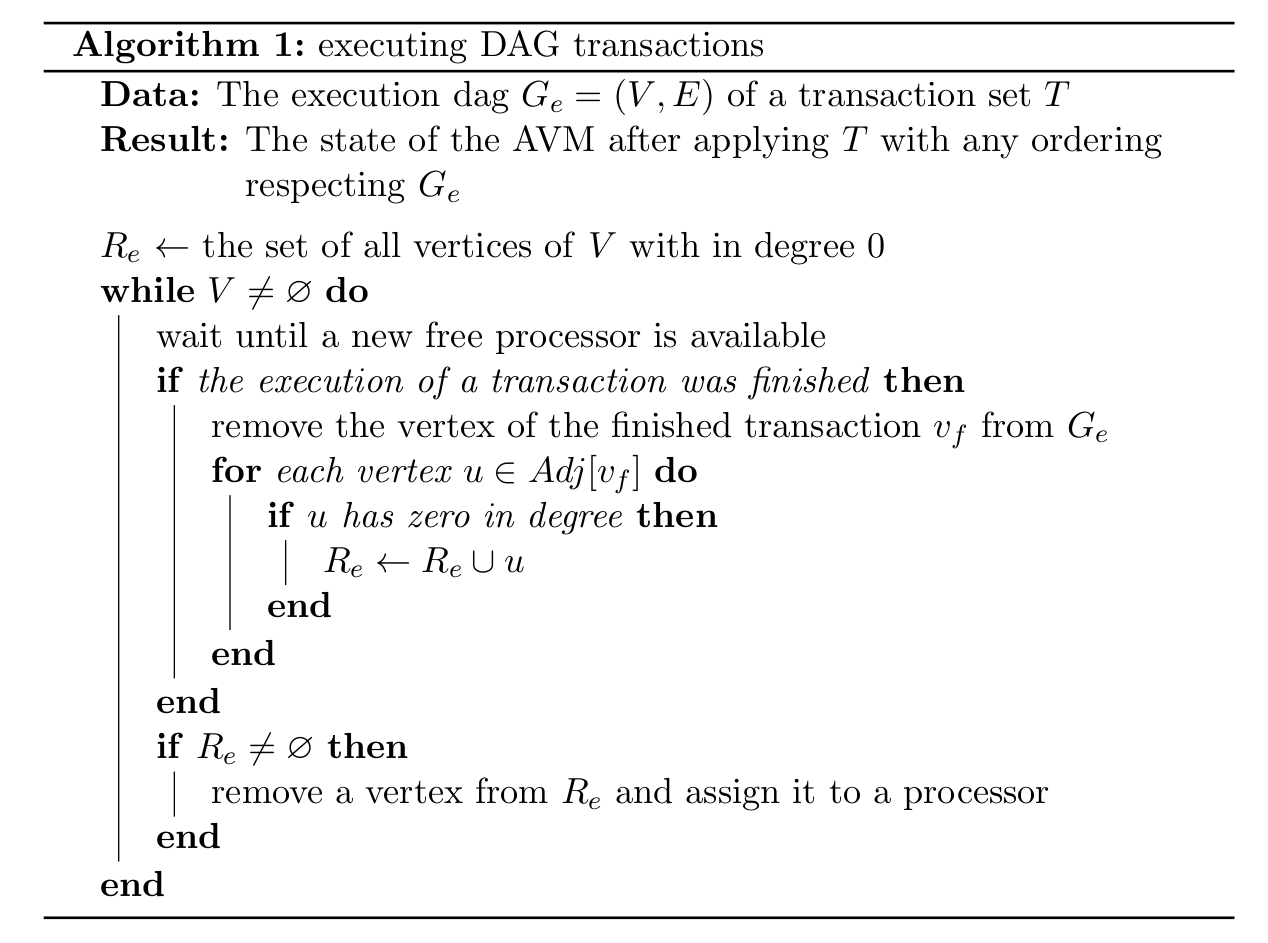
\includegraphics[width=17cm]{../img/Alg1.png}
    \begin{algorithm}
        \DontPrintSemicolon
        \SetKwData{Ready}{$R_e$}\SetKwData{V}{$v_f$}\SetKwData{Graph}{$G_e$}\SetKwData{Vertices}{$V$}\SetKwData
        {Txns}{$T$}
        \KwData{The execution dag $\Graph = (\Vertices,E)$ of a transaction set \Txns}
        \KwResult{The state of the AVM after applying \Txns with any ordering respecting \Graph}
        \BlankLine
        \Ready $\gets$ the set of all vertices of \Vertices with in degree 0\;
        \While{$\Vertices \neq \varnothing$}
        {
            wait until a new free processor is available\;
            \If{the execution of a transaction was finished}
            {
                remove the vertex of the finished transaction \V from \Graph\;
                \For{each vertex $u \in Adj[\V]$}
                {
                    \If{$u$ has zero in degree}
                    {
                        $\Ready \gets \Ready \cup u$\;
                    }
                }
            }
            \If{$\Ready \neq \varnothing$}
            {
                remove a vertex from \Ready and assign it to a processor\;
            }
        }
        \caption{executing DAG transactions}\label{alg:exec_dag}
    \end{algorithm}

    By replacing every undirected edge of a memory dependency graph with a directed edge in such a way that the
    resulted graph has no cycles, we will obtain a valid execution DAG. Thus, from a memory dependency graph different
    execution DAGs can be constructed with different levels of parallelization ability.

    If we assume that we have unlimited number of processors and all transactions take equal time for executing, it
    can be shown that by providing a minimal graph coloring to Algorithm~\ref{alg:gen_dag} as input, the resulted
    DAG will be optimal, in the sense that it results in the minimum overall execution time.

    %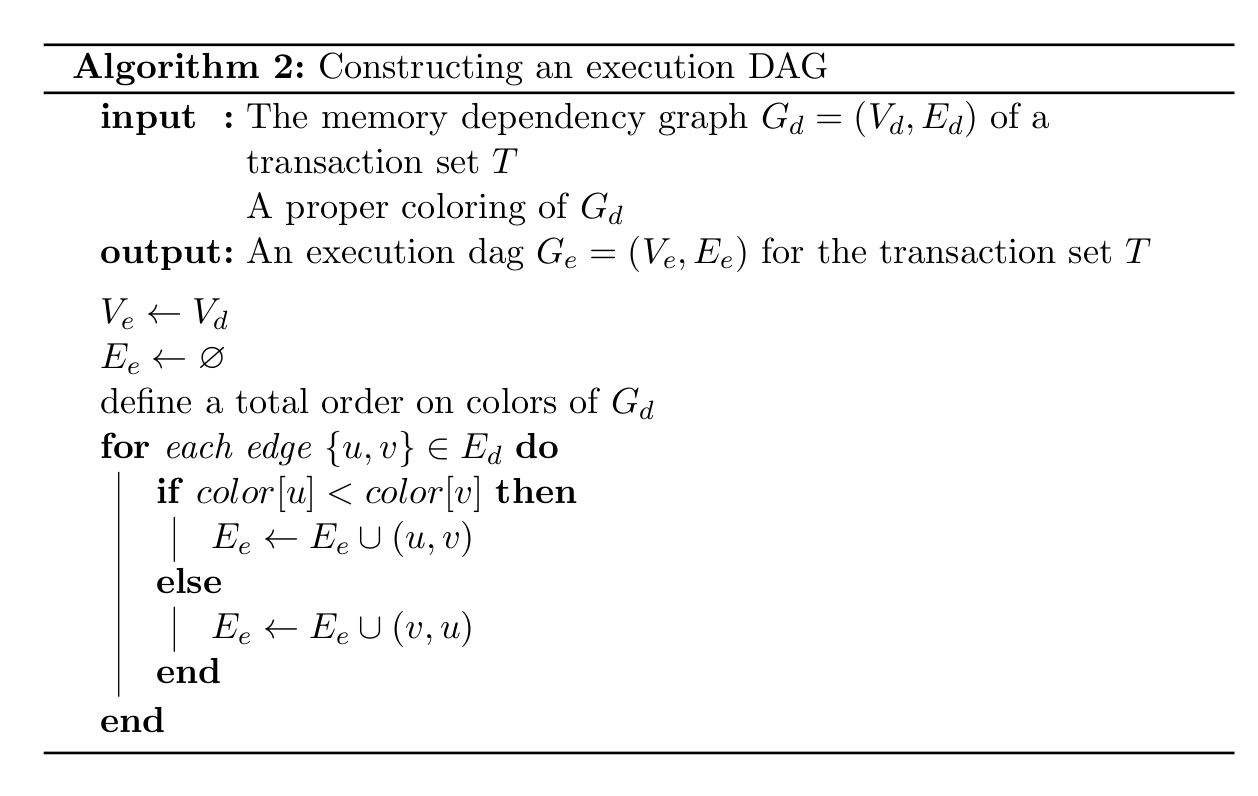
\includegraphics[width=17cm]{../img/Alg2.png}
    \begin{algorithm}
        \DontPrintSemicolon
        \SetKwData{Txns}{$T$}\SetKwData{Gd}{$G_d=(V_d,E_d)$}
        \SetKwInOut{Input}{input}\SetKwInOut{Output}{output}
        \Input{The memory dependency graph \Gd of a transaction set \Txns\\A proper coloring of $G_d$}
        \Output{An execution dag $G_e=(V_e,E_e)$ for the transaction set \Txns}
        \BlankLine
        $V_e \gets V_d$\;
        $E_e \gets \varnothing$\;
        define a total order on colors of $G_d$\;
        \For{each edge $\{u,v\} \in E_d$}
        {
            \eIf{$color[u] < color[v]$}
            {
                $E_e \gets E_e \cup (u,v)$\;
            }{
                $E_e \gets E_e \cup (v,u)$\;
            }
        }
        \caption{Constructing an execution DAG}\label{alg:gen_dag}
    \end{algorithm}

    The block proposer is responsible for proposing an efficient execution DAG alongside his proposed block which will
    determine the ordering of block transactions and help validators to validate transactions in parallel. Since with
    better parallelization a block can contain more transactions, a proposer is incentivized enough to find a good
    execution DAG for transactions.


 \subsection{Concurrent Counters}\label{subsec:concurrent-counters}

    We know that in Argennon every transaction needs to transfer its proposed fee to the \texttt{feeSink} accounts
    first. This essentially makes every transaction a reader and a writer of the memory locations which store the
    balance record of the \texttt{feeSink} accounts. As a result, all transactions in Argennon will be dependant and
    parallelism will be completely impossible. Actually, any account that is highly active, for example the account
    of an exchange or a payment processor, could become a concurrency bottleneck of the system, making all transactions
    which interact with them dependant.

    This problem can be easily solved by using a concurrent counter (CC) for storing the balance of this type of
    accounts. A concurrent counter is a data structure which improves concurrency by using multiple memory locations for
    storing a single counter. The value of the concurrent counter is equal to the sum of its sub counters and it can
    be incremented or decremented by incrementing/decrementing any of the sub counters. This way, a concurrent
    counter trades concurrency with memory usage.

    A pseudocode for implementing a concurrent counter (CC) which returns an error when the value of the counter
    becomes negative, follows:

    %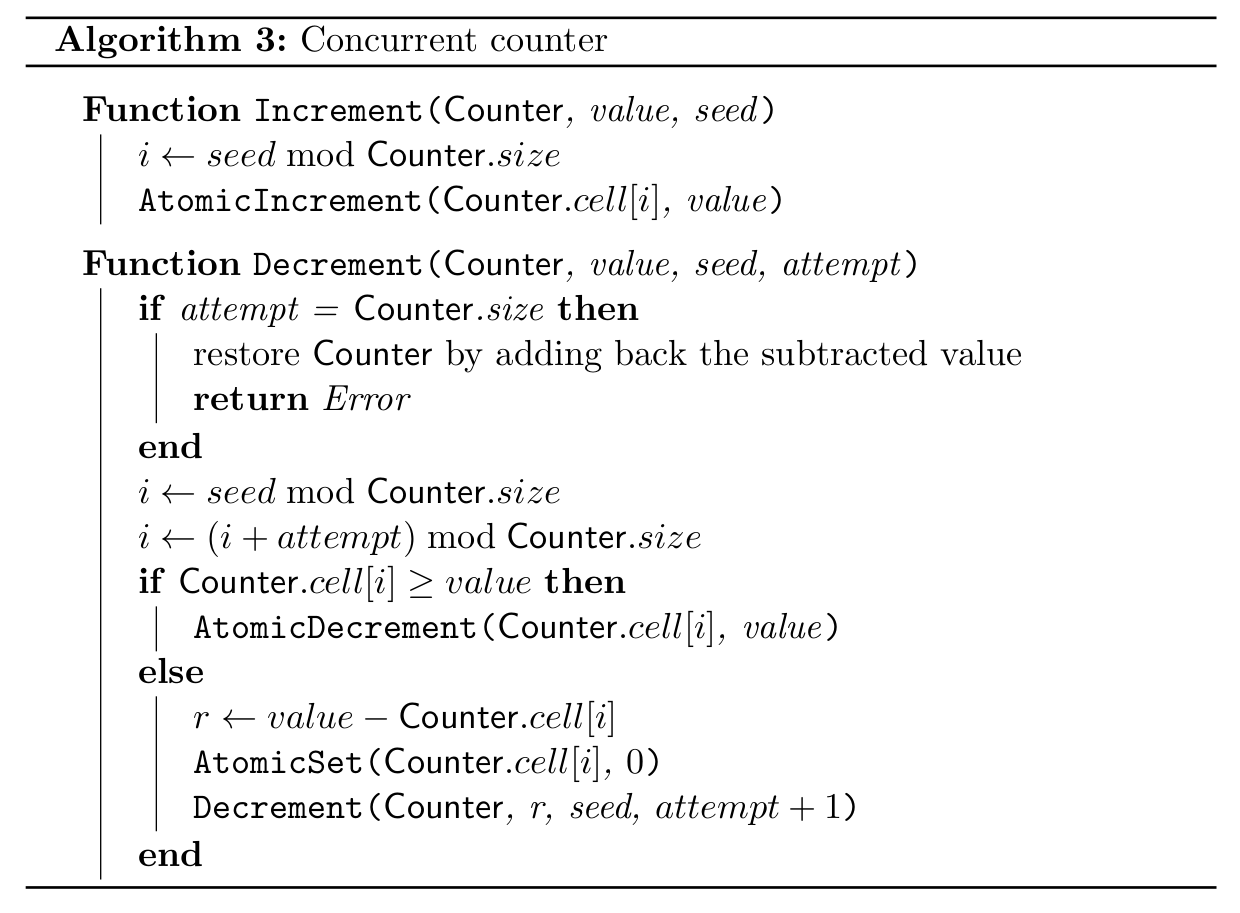
\includegraphics[width=17cm]{../img/Alg3.png}
    \begin{algorithm}
        \DontPrintSemicolon
        \SetKwData{CC}{Counter}
        \SetKwFunction{Inc}{Increment}\SetKwFunction{Dec}{Decrement}\SetKwFunction{AtomInc}{AtomicIncrement}
        \SetKwFunction{AtomDec}{AtomicDecrement}\SetKwFunction{AtomSet}{AtomicSet}
        \SetKwProg{Fn}{Function}{}{}
        \BlankLine
        \Fn{\Inc{\CC, value, seed}}
        {
            $i \gets seed \bmod \CC.size$\;
           \AtomInc{$\CC.cell[i]$, value}\;
        }
        \BlankLine
        \Fn{\Dec{\CC, value, seed, attempt}}
        {
            \If {attempt = \CC.size}
            {
                restore \CC by adding back the subtracted value\;
                \KwRet{Error}\;
            }
            $i \gets seed \bmod \CC.size$\;
            $i \gets (i + attempt) \bmod \CC.size$\;
            \eIf {$\CC.cell[i] \geq value$}
            {
                \AtomDec{$\CC.cell[i]$, value}\;
            }{
                $r \gets value - \CC.cell[i]$\;
                \AtomSet{$\CC.cell[i]$, $0$}\;
                \Dec{\CC, r, seed, $attempt + 1$}\;
            }
        }
        \caption{Concurrent counter}\label{alg:CC}
    \end{algorithm}

    It should be noted that in a blockchain application we don't have concurrent threads and therefore we don't need
    atomic functions. For usage in a smart contract, the atomic functions of this pseudocode can be implemented like
    normal functions.

    Concurrent counter data structure is a part of the AVM standard library, and any smart contract can use this data
    structure for storing the balance of highly active accounts.

    \subsection{Memory Chunks}\label{subsec:memory-chunks}

    In order to further increase the concurrency level of Argennon, we can divide the AVM memory into \emph{chunks}.
    Each memory chunk can be persisted using a different ZK-EDB, hence having its own commitment. Then, the
    consensus on new values of the commitment of any chunk can be achieved by different voting committees.

    If a transaction does not modify a memory chunk and in the transaction ordering of the block it comes after
    any transaction which modifies that chunk, then the execution of that transaction is not needed for calculating
    the new commitment of the chunk. Consequently, the voting committee of the memory chunk can safely ignore such a
    transaction. The execution DAG of transactions can be used for finding and pruning these transactions as
    we see in Algorithm~\ref{alg:prune_dag}.

    %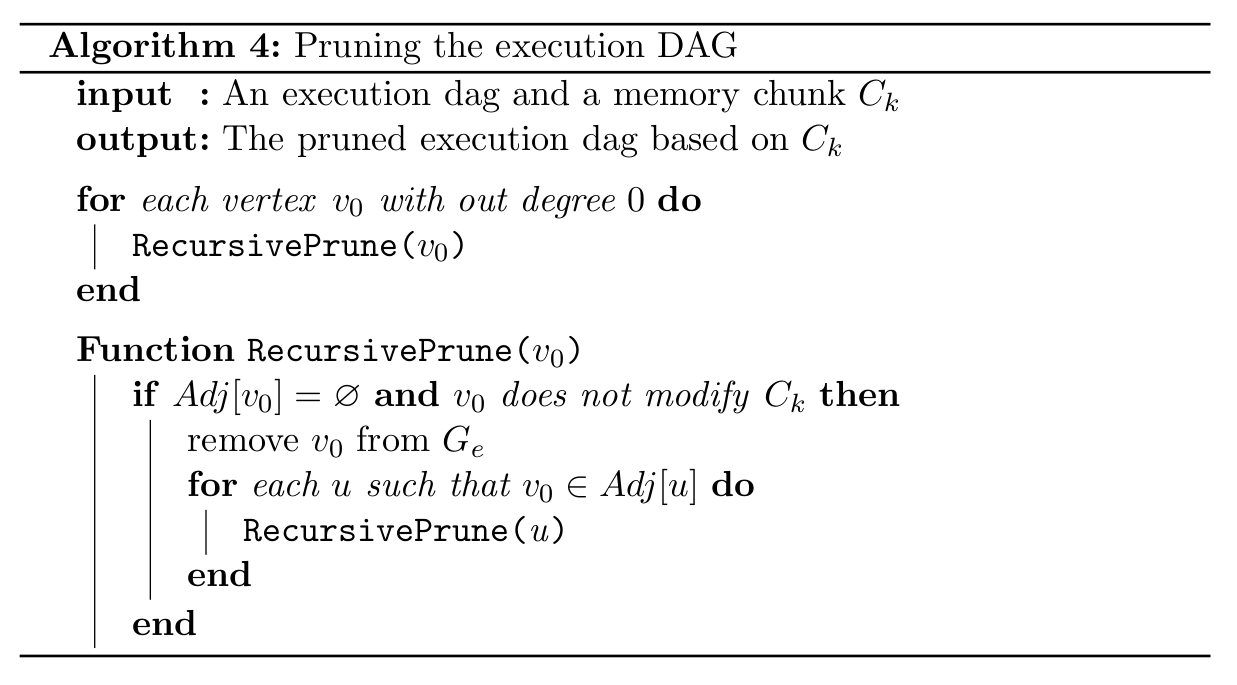
\includegraphics[width=17cm]{../img/Alg4.png}
    \begin{algorithm}
        \DontPrintSemicolon
        \SetKwData{V}{$v_0$}\SetKwData{Graph}{$G_e$}\SetKwData{Chunk}{$C_k$}\SetKwData{Txns}{$T$}
        \SetKwFunction{RPrune}{RecursivePrune}
        \SetKwProg{Fn}{Function}{}{}
        \SetKwInOut{Input}{input}\SetKwInOut{Output}{output}
        \Input{An execution dag and a memory chunk \Chunk}
        \Output{The pruned execution dag based on \Chunk}
        \BlankLine
        \For{each vertex \V with out degree $0$}
        {
            \RPrune{\V}\;
        }
        \BlankLine
        \Fn{\RPrune{\V}}
        {
            \If{$Adj[\V] = \varnothing$ {\bf and} \V does not modify \Chunk}
            {
                remove \V from \Graph\;
                \For{each $u$ such that $\V \in Adj[u]$}
                {
                    \RPrune{u}\;
                }
            }
        }
        \caption{Pruning the execution DAG}\label{alg:prune_dag}
    \end{algorithm}

    If we choose chunks in a way that most transactions only modify memory locations of one chunk,
    likely the transactions of a block are divided between voting committees and are validated in parallel.

    Because the voting committees are selected by random sampling, by choosing large enough samples we can make sure
    that having multiple voting committees will not change the security properties of the Argennon agreement protocol.

    \section{Consensus}\label{sec:consensus}

    The consensus protocol of Argennon is similar to Algorand with a few minor improvements.

    \subsection{Estimating A User's Stake}\label{subsec:estimating-a-user's-stake}

    In a proof of stake system the influence of a user in the consensus protocol should be proportional to the amount
    of stake the user has in the system. Conventionally in these systems, for estimating a user's stake, we use the
    amount of native system tokens the user is holding. Unfortunately, one problem with this approach is that a
    strong attacker may be able to obtain a considerable amount of system tokens, for example by borrowing from a
    DEFI application, and use this stake to attack the system.

    To mitigate this problem, for calculating a user's stake at the time step \(t\), instead of using the raw ARG
    balance, we use the minimum of a \emph{trust value} the system has calculated for the user and the user's
    ARG balance:
    \[
        S_{u,t} = \min (B_{u,t}, Trust_{u,t})
    \]
    Where:
    \begin{itemize}
        \item \(S_{u,t}\) is the stake of the user \(u\) at the time step \(t\).
        \item \(B_{u,t}\) is the ARG balance of the user \(u\) at the time step \(t\).
        \item \(Trust_{u,t}\) is an estimated trust value for the user \(u\) at the time step \(t\).
    \end{itemize}

    The agreement protocol, at the time step \(t\), will use \(\sum_{u}S_{u,t}\) to determine the required
    number of votes for the confirmation of a block, and we let \(Trust_{u,t} = M_{u,t}\), where \(M_{u,t}\) is the
    exponential moving average of the ARG balance of the user \(u\) at the time step \(t\).

    In our system a user who held ARGs and participated in the consensus for a long time is more trusted
    than a user with a higher balance whose balance has increased recently. An attacker who has obtained a large
    amount of ARGs, also needs to hold them for a long period of time before being able to attack the system.

    For calculating the exponential moving average of a user's balance at the time step \(t\), we can use the following
    recursive formula:
    \[
        M_{u,t} = (1 - \alpha) M_{u,t-1} + \alpha B_{u,t} = M_{u,t-1} + \alpha (B_{u,t} - M_{u,t-1})
    \]
    Where the coefficient \(\alpha\) is a constant smoothing factor between \(0\) and \(1\) which represents the
    degree of weighting decrease, A higher \(\alpha\) discounts older observations faster.

    Usually an account balance will not change in every time step, and we can use older values of EMA for calculating
    \(M_{u,t}\): (In the following equations the \(u\) subscript is dropped for simplicity)
    \[
        M_{t} = (1 - \alpha)^{t-k}M_{k} + [1 - (1 - \alpha)^{t - k}]B
    \]
    Where:
    \[
        B = B_{k+1} = B_{k+2} = \dots = B_{t}
    \]
    We know that when \(|nx| \ll 1\) we can use the binomial approximation \({(1 + x)^n \approx 1 + nx}\). So, we can
    further simplify this formula:
    \[
        M_{t} = M_{k} + (t - k) \alpha (B - M_{k})
    \]

    For choosing the value of \(\alpha\) we can consider the number of time steps that the trust value of a user needs
    for reaching a specified fraction of his account balance. We know that for large \(n\) and \(|x| < 1\) we have
    \((1 + x)^n \approx e^{nx}\), so by letting \(M_{u,k} = 0\) and \(n = t - k\) we can write:
    \[
        \alpha =- \frac{\ln\left(1 - \frac{M_{n+k}}{B}\right)}{n}
    \]
    The value of \(\alpha\) for a desired configuration can be calculated by this equation. For instance, we could
    calculate the \(\alpha\) for a relatively good configuration in which \(M_{n+k} = 0.8B\) and \(n\) equals to the
    number of time steps of 10 years.

    In our system a newly created account will not have voting power for some time, no matter how high its
    balance is. While this is a desirable property, in case a large proportion of total system tokens are
    transferred to newly created accounts, it can result in too much voting power for older accounts. This may decrease
    the degree of decentralization in our system.

    However, this situation is easily detectable by comparing the total stake of the system with the total balance of
    users. If after confirming a block the total stake of the system goes too low and we have:
    \[
        \sum_{u}S_{u,t} < \gamma \sum_{u}B_{u,t}
    \]
    The protocol will perform a \emph{time shift} in the system: the time step of the system
    will be incremented for \(m\) steps while no blocks will be confirmed. This will increase the value of \(M_{u,t}\)
    for new accounts with a non-zero balance, giving them more influence in the agreement protocol.

    For calculating the value of \(m\) which determines the amount of time shift in the system, we should note that when
    \(B_{u,t} = B_{u, t-1} = B_u\), we can derive a simple recursive rule for the stake of a user:
    \[
        S_{u,t} = (1 - \alpha) S_{u,t-1} + \alpha B_u
    \]
    Therefore, we have:
    \[
        \sum_{u}S_{u,t} = (1 - \alpha) \sum_{u}S_{u,t - 1} + \alpha \sum_{u}B_u
    \]
    This equation shows that when the balance of users is not changing over time the total stake of the system is the
    exponential average of the total ARGs of the system. Consequently, when we shift the time for \(m\) steps, we can
    calculate the new total stake of the system from the following equation:

    \[
        \sum_{u}S_{u,t+m} = (1 - \alpha)^{m}\sum_{u}S_{u,t} + [1 - (1 - \alpha)^{m}]\sum_{u}B_u
    \]
    Hence, if we want to increase the total stake of the system from \(\gamma \sum_{u}B_u\) to \(\lambda \sum_{u}B_u\),
    we can obtain \(m\) from the following formula, assuming \(\alpha\) is small enough:
    \[
        m = \frac{1}{\alpha} \ln \left(\frac{1 - \gamma}{1 - \lambda}\right)
    \]


    \section{Smart Contract Oracle}\label{sec:smart-contract-oracle}

    A smart contract oracle is a full AVM emulator that keeps a full local copy of AVM memory and can emulate AVM
    execution without accessing a ZK-EDB. Smart contract oracles can be used for reporting useful information about
    \texttt{avmCall} transactions such as accessed AVM heap or code area locations, exact amount of execution cost,
    and so on.

\end{document}


